\newcommand{\PartieI}{Partie I : L'algorithme de recommandation basé sur la factorisation matricielle}
\definecolor{darkgreen}{RGB}{0,100,0}

\begin{frame}{Sommaire}
    \begin{itemize}
        \item Introduction
        \item \textbf{L'algorithme de recommandation basé sur la factorisation matricielle}
    \end{itemize}
\end{frame}

\begin{frame}{\PartieI}
    \begin{itemize}
        \item Faisant partie du filtrage collaboratif...
        \item {
              Ce dont on dispose :
              \begin{figure}[htbp]
                  \centering
                  \hspace{80pt}
                  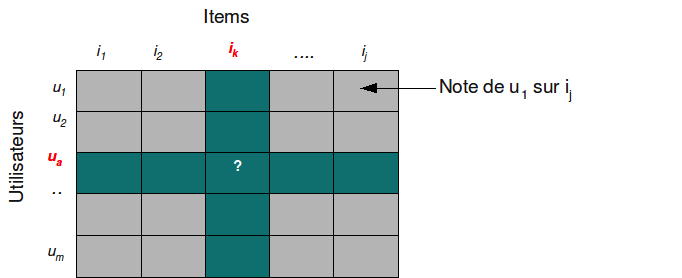
\includegraphics[width=0.6\textwidth]{PartieI/matrix_users_items.png}
                  \caption{Matrice utilisateur-article notée $\mathcal{R}$}
                  \label{fig:matrix-user-article}
              \end{figure}
              }
    \end{itemize}
\end{frame}

\begin{frame}{\PartieI}
    \begin{center}
        \textcolor{red}{\textbf{\large{Problème !!}}}
    \end{center}
\end{frame}

\begin{frame}{\PartieI}
    \begin{center}
        \textcolor{darkgreen}{\textbf{\large{Factorisation Matricielle}}}
    \end{center}
\end{frame}

\begin{frame}{\PartieI}
    On note :
    \begin{itemize}
        \item $\mathcal{R}$ comme la matrice originale de taille $m \times n$, où $m$ est le nombre d'utilisateurs et $n$ est le nombre d'articles.
        \item $\mathcal{P}$ comme la matrice d'utilisateurs de taille $m \times k$, où $k$ est le nombre de facteurs latents.
        \item $\mathcal{Q}$ comme la matrice d'articles de taille $k \times n$.
    \end{itemize}
    \begin{center}
        \textbf{L'objectif est de trouver P et Q tels que R = PQ.}
    \end{center}
\end{frame}

\begin{frame}{\PartieI}
    L'erreur quadratique moyenne est donnée par :
    \begin{equation*}
        \mathrm{EQM}=\frac{1}{m \times n} \sum_{i=1}^m \sum_{j=1}^n\left(R_{i j}-(P Q)_{i j}\right)^2
    \end{equation*}

\end{frame}

\begin{frame}{\PartieI}
    La fonction de perte avec régularisation est donnée par :
    \begin{equation*}
        \text { Perte }=\frac{1}{m \times n} \sum_{i=1}^m \sum_{j=1}^n\left(R_{i j}-(P Q)_{i j}\right)^2+\lambda\left(||P||^2+||Q||^2\right)
    \end{equation*}
    où $\lambda$ est le facteur de régularisation, et $\|P\|^2$ et $\|Q\|^2$ sont les normes de Frobenius de $P$ et $Q$, respectivement.
\end{frame}

\begin{frame}{\PartieI}
    La méthode de descente de gradient stochastique (DGS) se fait avec :
    \begin{equation*}
        P_{i k}=P_{i k}+\alpha\left(e_{i j} Q_{k j}-\lambda P_{i k}\right)
    \end{equation*}
    \begin{equation*}
        Q_{k j}=Q_{k j}+\alpha\left(e_{i j} P_{i k}-\lambda Q_{k j}\right)
    \end{equation*}
    où $e_{i j}=R_{i j}-\sum_k P_{i k} Q_{k j}$ est l'erreur de prédiction pour l'élément $R_{i j}$ de la matrice de notation.
\end{frame}

\begin{frame}{\PartieI}
    \begin{center}
        \textbf{\large{Les \textcolor{darkgreen}{avantages} et les \textcolor{red}{limites} de la méthode de descente de gradient stochastique (DGS)}}
    \end{center}
\end{frame}

\begin{frame}{\PartieI}
    \begin{center}
        \large{Une alternative : \textbf{La méthode des moindres carrés alternés (MCA)}}
    \end{center}
\end{frame}

\begin{frame}{\PartieI}
    \begin{center}
        \textbf{\large{Les \textcolor{darkgreen}{avantages} et les \textcolor{red}{limites} de la méthode des moindres carrés alternés (MCA)}}
    \end{center}
\end{frame}

\begin{frame}{\PartieI}
    \begin{center}
        \textbf{\large{Les \textcolor{darkgreen}{avantages} et les \textcolor{red}{limites} de la factorisation matricielle}}
    \end{center}
\end{frame}